\documentclass[a4paper, 11pt]{article}
\usepackage{geometry}
\geometry{letterpaper, margin=1in}
\usepackage{amsmath}
\usepackage{amssymb}  
\usepackage{amsthm}
\usepackage{ulem} 
\usepackage{graphicx}
\usepackage{enumitem} 
\graphicspath{ {images/} }


\newtheorem*{theorem}{Theorem}

\begin{document}
%Header-Make sure you update this information!!!!
\noindent
\large\textbf{Complex Analysis: Day 18} \hfill \textbf{John Waczak} \\
\normalsize MTH 483 \hfill  Date: \today \\

\subsection*{More power series stuff} 
	If $f(z)=\sum\limits_{n=0}^{\infty} a_n(z-c)^n$ has radius of convergence R, then it defines a holomorphic function on the disc $|z-c|<R$. (If $R=+\infty$ then the function is entire). Moreover:
		\begin{equation*}
			f'(z) = \sum\limits_{n=1}^\infty a_n n (z-c)^{n-1}
		\end{equation*}
	
	\noindent which has the same radius of convergence $\sqrt[n]{n}\rightarrow 1$ as $n\rightarrow \infty$. Thus  by reapplication of the theorem to subsequent derivatives we have that $f(z)$ has infinitely many derivatives. \\
	
	\noindent A useful formula is:
		\begin{align*}
			a_n &= \frac{f^{(n)}(c)}{n!} \\ 
			f(z) &= \sum\limits_{k=0}^{\infty} a_k(z-c)^k \\ 
			f'(z) &= \sum\limits_{k=1}^{\infty} a_k(k)(z-c)^{k-1} \\
			 &. \\ 
			 &. \\ 
			 &. \\ 
			f^{(n)}(z) &= \sum\limits_{k=n}^\infty a_k k(k-1)(k-2)...(k-(n-1))(z-c)^{k-n}
		\end{align*}
	\noindent So it seems like functions that can be written as power-series are infinitely better than just our regular holomorphic functions. \\ 
	
	\begin{theorem}
		Let $f:\Omega\rightarrow\mathbb{C}$ be holomorphic and let $c\in\Omega$, $R>0$ for which $D_R(c)\subseteq\Omega$. Then f can be represented as a power series:
			\begin{equation*}
				f(z) = \sum\limits_{n=0}^{\infty} a_n(z-c)^n 
			\end{equation*}
		for all $z\in D_R(c)$. Moreover, the radius of convergence of the power series is $\geq R$. Finally, the coefficient $a_n$ is given by $a_n = \frac{f^{(n)}(c)}{n!}$. 
	\end{theorem}
	
	\noindent You might ask what is the difference between a Taylor and power series? A power series is a function defined by the infinite sum. A Taylor series is when we start with a function and then define the $a_n$'s in the sum. For us they are essentially the same thing. \\ 
	
	\begin{figure}[!hbt]
		\centering
		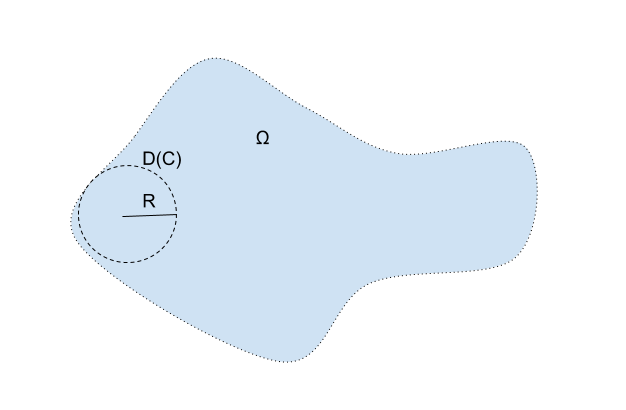
\includegraphics[scale=0.5]{powerSeriesDisc}
	\end{figure}
	
	
	\begin{proof}
		Main ingredient: Cauchy's integral formula. Take $c=0$ for simplicity. Given $z\in D_R(0)$, define r so that $r=\frac{|z|+R}{2}$ and $D_{r}(0)\subseteq D_R(0)$. By CIF we have that: 
			\begin{align*}
				f(z) &= \frac{1}{2\pi i}\oint_{|w|=r}\frac{f(w)}{w-z}dw\\ 
					&= \frac{1}{2\pi i}\oint_{|w|=r} \frac{f(w)}{w(1-\frac{z}{w})}dw\\
				\text{now } |z/w| &= |z|/r < 1 \\ 
					&= \frac{1}{2\pi i}\oint_{|z|=r}\frac{f(w)}{w}\sum\limits_{k=0}^\infty \Big(\frac{z}{w}\Big)^k dw \\ 
					&= \sum\limits_{k=0}^\infty  \Bigg\{ \frac{1}{2\pi i}\oint_{|z|=r} \frac{f(w)}{w^{k+1}} dw \Bigg\}z^k \\ 
				\text{let } a_k &= \frac{1}{2\pi i}\oint_{|w|=r}\frac{f(w)}{w^{k+1}}dw \\ 
			\end{align*}
	\end{proof}
	
	\begin{theorem}[Corollary]
		Let $f:\Omega\rightarrow \mathbb{C}$ be holomorphic and let $c\in\Omega$, then the power series for $f(z)$ given by 	
			\begin{equation*}
				f(z) = \sum\limits_{n=0}^\infty \frac{f^{(n)}(c)}{n!}(z-c)^n
			\end{equation*}
		has radius of convergence at least the distance from c to the nearest point on the boundary of $\Omega$. 
	\end{theorem}
	
	
	
	
	
	
	
	
	
	
	
	
	
	
	
	
	
	
\end{document}




















